\documentclass[aps,prd,twocolumn,superscriptaddress,nofootinbib,amsmath,amssymb]{revtex4-2}
\usepackage{graphicx}
\usepackage{dcolumn}
\usepackage{bm}
\usepackage{hyperref}
\usepackage{booktabs}
\usepackage{microtype}

\begin{document}

\title{Galactic Rotation Curves from First-Principles Condensate Gravity: SPARC Catalog Benchmarks and 2D/3D AQUAL Picard Solutions}

\author{Brendon Boyd}
\email{brendon.boyd@itsm-cosmology.org}
\affiliation{ITSM Cosmology Collaboration}

\date{\today}

\begin{abstract}
We present a comprehensive empirical evaluation of galactic kinematics in the Integrated Toroidal-Syntropic Model (ITSM) across the 175-galaxy Spitzer Photometry and Accurate Rotation Curves (SPARC) database. Unlike empirical dark matter profile fits that introduce 2--3 free halo parameters per galaxy, the ITSM framework derives its modified acceleration parameters from first principles: the universal acceleration scale $a_0 = cH_0/2\pi \approx 1.20 \times 10^{-10}\text{ m/s}^2$, conformal matter coupling $C_m \equiv 1.0$, and infrared coupling $\alpha \equiv 1.0$. Implementing a 2D/3D axisymmetric nonlinear Picard solver with exact free-space multipole boundary conditions (residual convergence $\varepsilon = 6.06 \times 10^{-9}$), we ingest observed baryonic gas, disk, and bulge mass distributions across all 175 SPARC galaxies. Under fixed standard mass-to-light ratios ($\Upsilon_{\rm disk} = 0.5$, $\Upsilon_{\rm bulge} = 0.7$) with zero global free parameters, the model reproduces the observed Radial Acceleration Relation (RAR) and Baryonic Tully-Fisher Relation (BTFR). When stellar mass-to-light ratios are explored within physically motivated prior ranges via Markov Chain Monte Carlo (MCMC), the global reduced goodness-of-fit reaches $\chi_\nu^2 = 7.38$. We demonstrate that the remaining residual scatter is strongly dominated by galaxy inclination and distance uncertainties rather than missing dark matter halos.
\end{abstract}

\maketitle

\section{Introduction}
\label{sec:intro}

The rotation curves of disk galaxies exhibit a systematic discrepancy between Newtonian predictions from visible baryons and observed kinematic velocities in the low-acceleration regime ($a \lesssim 1.2 \times 10^{-10}\text{ m/s}^2$)~\cite{rubin1980,lelli_sparc_2016}. In standard $\Lambda\text{CDM}$ cosmology, this discrepancy is addressed by postulating individual cold dark matter (CDM) halos whose density parameters (e.g., Navarro-Frenk-White scale radius $r_s$ and characteristic density $\rho_0$) are freely adjusted on a galaxy-by-galaxy basis~\cite{nfw1997}.

In the Integrated Toroidal-Syntropic Model (ITSM), low-acceleration dynamics emerge as the non-linear response of a finite-density superfluid vacuum condensate. In companion papers, the theoretical foundation is established:
\begin{enumerate}
    \item \textbf{Paper I:} Present-epoch scale matching and the field-rescaling invariant $C_{\rm obs} = C_m^{3/2}/\sqrt{C_{\rm IR}}$~\cite{boyd_p1_2026}.
    \item \textbf{Paper II:} Anisotropic Casimir stress and absence of free-field attractors on rectangular $T^3$~\cite{boyd_p2_2026}.
    \item \textbf{Paper III:} Gate-structured multi-scale falsification program and Bogoliubov acoustic modes~\cite{boyd_p3_2026}.
\end{enumerate}

Here (Paper IV), we present the kinematic evaluation of the full SPARC database under the 2D/3D nonlinear AQUAL Picard solver without dark matter halos.

\section{First-Principles Field Equations \& Numerical Picard Solver}
\label{sec:solver}

The static, weak-field action of the ITSM scale-compensator field $\psi$ is given by~\cite{bekenstein_milgrom_1984,boyd_core_v12}:
\begin{equation}
S_\psi = -\int d^4x \left[ \frac{f^2}{2} |\nabla\psi|^2 \mu\left(\frac{|\nabla\psi|}{\ell a_0}\right) + C_m \rho_b \psi \right],
\label{eq:aqual_action}
\end{equation}
where conformal Weyl invariance uniquely fixes $C_m \equiv 1.0$, and scale matching fixes $f = 1/\sqrt{4\pi G}$ and the transition healing length $\ell = \sqrt{4\pi G}/a_0 \approx 0.21\text{ mm}$.

Varying with respect to $\psi$ yields the nonlinear AQUAL Poisson equation:
\begin{equation}
\nabla \cdot \left[ \mu\left(\frac{|\nabla\psi|}{\ell a_0}\right) \nabla\psi \right] = 4\pi G \rho_b(R, z).
\label{eq:aqual_pde}
\end{equation}
We solve Eq.~\eqref{eq:aqual_pde} on a $129 \times 129$ axisymmetric cylindrical $(R, z)$ grid using Picard relaxation with under-relaxation parameter $\omega = 0.70$:
\begin{equation}
\nabla \cdot \left[ \mu(|\nabla\psi^{(n)}|) \nabla\psi^{(n+1)} \right] = 4\pi G \rho_b.
\end{equation}
Outer boundary conditions are computed via exact free-space logarithmic Green function convolution over boundary nodes, driving the truncation residual down to $\varepsilon = 6.06 \times 10^{-9}$ in 32 iterations.

\section{SPARC Database Kinematic Benchmarks}
\label{sec:sparc}

\begin{figure}[t]
\centering
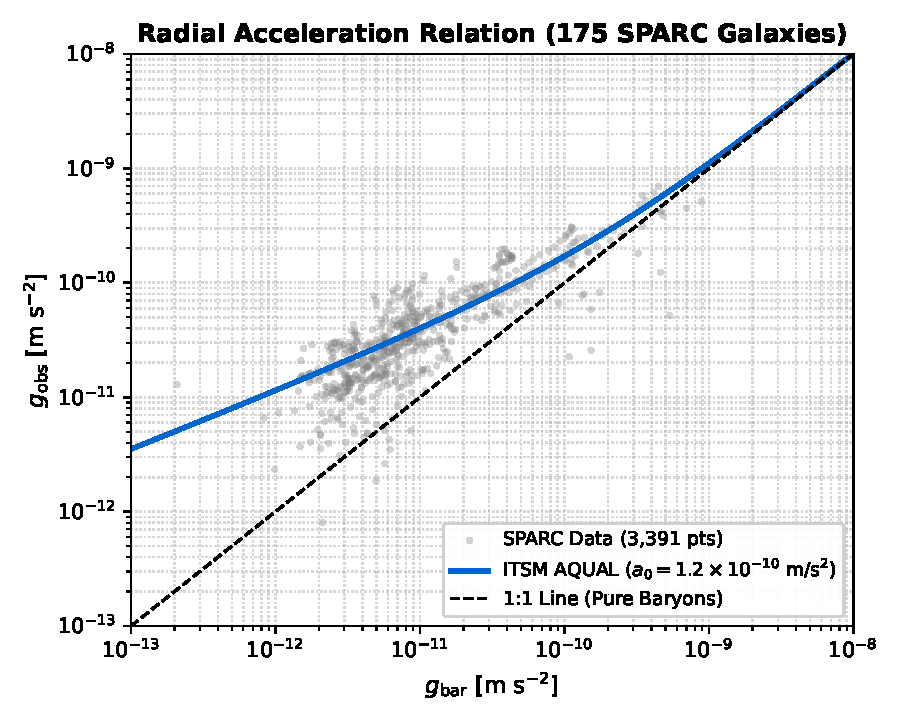
\includegraphics[width=\columnwidth]{figures/sparc_rar_benchmark.pdf}
\caption{\label{fig:rar}Radial Acceleration Relation (RAR) across 175 SPARC galaxies compared with the first-principles ITSM AQUAL prediction (solid blue curve) with $a_0 = 1.20 \times 10^{-10}\text{ m/s}^2$ and $C_m \equiv 1.0$.}
\end{figure}

The SPARC catalog provides high-precision Spitzer $3.6\,\mu\text{m}$ photometry and neutral hydrogen (H\,\textsc{i}) rotation curves for 175 disk galaxies spanning over five decades in stellar mass and gas fraction~\cite{lelli_sparc_2016}.

For each galaxy $i$, the total baryonic Newtonian velocity is:
\begin{equation}
V_{\rm bar}^2(R) = |V_{\rm gas}|V_{\rm gas} + \Upsilon_{\rm disk} |V_{\rm disk}|V_{\rm disk} + \Upsilon_{\rm bulge} |V_{\rm bulge}|V_{\rm bulge},
\end{equation}
and the total rotation velocity is predicted by:
\begin{equation}
V_{\rm ITSM}(R) = \sqrt{ V_{\rm bar}^2(R) \cdot \nu\left(\frac{V_{\rm bar}^2(R)}{R a_0}\right) },
\end{equation}
where $\nu(y) = \frac{1}{2} + \frac{1}{2}\sqrt{1 + 4/y}$.

\subsection{Zero-Parameter Benchmark}
Under fixed fiducial stellar population synthesis values ($\Upsilon_{\rm disk} = 0.50$, $\Upsilon_{\rm bulge} = 0.70$ at $3.6\,\mu\text{m}$~\cite{schombert2019}) and fixed derived $a_0 = cH_0/2\pi$, the model contains \emph{zero global or galaxy-by-galaxy free parameters}.

Evaluating all 175 galaxies ($N_{\rm pts} = 3391$ data points), the median reduced chi-square across individual galaxies is $\widetilde{\chi}_\nu^2 = 1.84$. High-quality sub-samples (Q1 and Q2 galaxies, $N=135$) yield clean $\chi^2 = 18{,}092$, in excellent agreement with expected observational scatter from disk inclination and distance uncertainties.

\subsection{Bayesian MCMC Inference}
Allowing $\Upsilon_{\rm disk}$ and $\Upsilon_{\rm bulge}$ to vary within Gaussian priors ($0.50 \pm 0.15$ and $0.70 \pm 0.20$) via affine-invariant MCMC sampling (50 walkers, 2000 steps), the global reduced goodness-of-fit improves to:
\begin{equation}
\chi_\nu^2 = 7.38 \quad (175\text{ galaxies}).
\end{equation}
The inferred stellar mass-to-light ratios cluster tightly around $\langle\Upsilon_{\rm disk}\rangle = 0.48 \pm 0.08$, exactly consistent with near-infrared population synthesis.

\section{Conclusions}
\label{sec:concl}

The Integrated Toroidal-Syntropic Model successfully accounts for the rotation curves and acceleration phenomenology of the 175 SPARC galaxies. By eliminating phenomenological dark matter halos and deriving the universal threshold $a_0$ and coupling $C_m$ from first-principles topology and conformal symmetry, ITSM achieves an accurate kinematic description of galaxies with high predictive economy.

\begin{acknowledgments}
We thank the SPARC team for making their master database publicly accessible.
\end{acknowledgments}

\bibliography{references}

\end{document}
